\section{Технический проект}
\subsection{Общая характеристика организации решения задачи}

Для реализации поставленных задач необходимо спроектировать и разработать программно-информационную систему, включающую в себя реляционную базу данных и приложение с интерфейсом для взаимодействия ней.

\subsection{Обоснование выбора технологии проектирования}

Используемые для создания программно-информационной системы языки и технологии отвечают современным практикам разработки, позволяют достичь высокой производительности и отказоустойчивости программы.

\subsubsection{Язык программирования Python}

В качестве основного языка программирования выбран Python, благодаря его сочетанию выразительности, гибкости и обширной поддержки со стороны сообщества разработчиков. Python — это высокоуровневый, интерпретируемый язык, активно применяющийся как в образовательных, так и в промышленных проектах. Основные причины выбора языка заключаются в следующем:
\begin{enumerate}
	\item Простой и интуитивно понятный синтаксис значительно сокращает порог вхождения и снижает количество потенциальных ошибок при написании кода. Это особенно важно в условиях ограниченного времени на разработку и тестирование, а также при передаче проекта на сопровождение.
	\item Поддержка нескольких парадигм программирования, включая объектно-ориентированную, процедурную и функциональную, делает Python универсальным инструментом. Это позволяет организовать код в соответствии с принципами модульности, инкапсуляции и повторного использования.
	\item Обширная стандартная библиотека и внешняя экосистема обеспечивают доступ к готовым модулям для сериализации, построения интерфейса, анализа синтаксических деревьев, многопоточности и многого другого. Это существенно ускоряет разработку и упрощает реализацию сложных функций.
	\item Кроссплатформенность языка позволяет запускать приложение на операционных системах Windows, Linux и macOS без необходимости адаптации кода под конкретную платформу. Таким образом, обеспечивается максимальная универсальность и доступность системы для пользователя.	
\end{enumerate}
Таким образом, Python представляет собой оптимальное решение для реализации проекта, сочетающее в себе простоту, мощь и гибкость, что делает его незаменимым инструментом в учебных и практических задачах программной инженерии.

\subsubsection{Графический интерфейс с использованием tkinter}

Для построения графического интерфейса выбрана встроенная библиотека tkinter.

Tkinter полностью удовлетворяет требованиям к простому, лёгкому в использовании, но функциональному графическому интерфейсу.

\subsubsection{Обработка выражений с использованием ast}

Обработка запросов реализована с использованием модуля ast из стандартной библиотеки Python.

\subsubsection{Сериализация и хранение с использованием pickle}

Для хранения базы данных используется механизм сериализации объектов с помощью модуля pickle, который входит в стандартную библиотеку Python.

\subsection{Архитектура программной системы}

На рисунке ~\ref{fig:architecture} в виде UML-диаграммы представлена архитектура программной системы.
\begin{figure}[H]
	\centering
	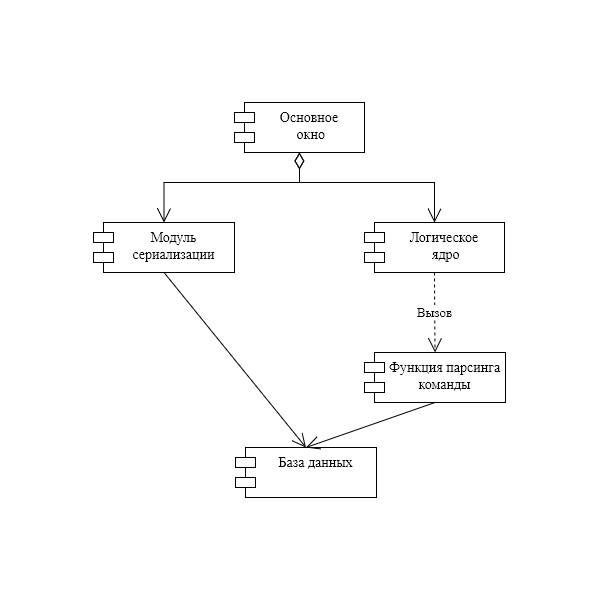
\includegraphics[width=1\linewidth]{images/architecture}
	\caption{Архитектура программной системы}
	\label{fig:architecture}
\end{figure}

\subsubsection{Общая структура системы}

Программа условно разделена на четыре компонента:
\begin{enumerate}
	\item Логическое ядро — реализует логику обработки команд, взаимодействие с внутренним представлением базы данных, интерпретацию пользовательского ввода и выполнение операций (select, insert, delete, update и др.).
	\item Графическая оболочка — отвечает за взаимодействие с пользователем через визуальный интерфейс, реализованный с использованием библиотеки tkinter.
	\item База данных -- реализованная средствами Python реляционная модель, предназначенная для хранения данных.
	\item Модуль хранения и сериализации — обеспечивает сохранение состояния базы данных в бинарном виде и восстановление при запуске программы с использованием стандартного модуля pickle.
\end{enumerate}

\subsubsection{Поток выполнения и взаимодействие компонентов}

Система построена по модульной архитектуре с явным разделением ответственности между компонентами. Все модули взаимодействуют по иерархии "<сверху вниз">:
\begin{enumerate}
	\item Пользователь взаимодействует с приложением через графическую оболочку. Эта оболочка содержит обработчики событий, виджеты (таблицу, формы, кнопки, поле ввода) и элементы навигации.
	\item Графическая оболочка передаёт все команды и параметры непосредственно в логическое ядро, которое выступает в роли контроллера и интерпретатора команд.
	\item Логическое ядро реализует	интерпретацию пользовательских команд (анализ строк, парсинг) и проводит операции с таблицами: фильтрацию, выборку, обновление, удаление и т.п. 
	\item Вся информация хранится в внутренней модели данных, которая представляет таблицы как структуры на основе словарей и списков.
	\item Для долговременного хранения используется модуль сериализации, основанный на pickle. Он обеспечивает сохранение всей модели данных в бинарный файл при выходе из приложения и её восстановление при следующем запуске.
\end{enumerate}

\subsection{Архитектура приложения}

Точкой входа в программу является модуль main.py, в котором создаётся и запускается экземпляр класса MainWindow, реализующего основной графический интерфейс приложения.

Архитектура приложения состоит из следующих ключевых модулей:
\begin{enumerate}
	\item main.py — стартовый модуль, в котором производится инициализация пользовательского интерфейса. Здесь создаётся объект MainWindow, который затем запускается методом mainloop(). Этот файл минимален по содержанию и служит точкой входа в приложение.
	\item dbwindow.py — содержит основной класс пользовательского интерфейса MainWindow, реализованный с использованием библиотеки tkinter. Класс отвечает за построение структуры окна и визуальное отображение таблиц. Взаимодействие с моделью данных и логическим ядром осуществляется через внутренние методы и обработчики событий.
	\item database.py — реализует класс Database, представляющий собой структуру хранения данных. Он содержит таблицы в виде словарей и предоставляет методы добавления, удаления, выборки и сериализации данных.
	\item table.py — содержит реализацию класса Table, представляющего одну таблицу базы данных. Класс обеспечивает работу с полями и строками, а также поддерживает базовые операции (insert, delete, update, select), реализуемые как на уровне структуры, так и логически. Этот класс тесно взаимодействует с логическим ядром, обеспечивая доступ к данным.
	\item parser.py —  обрабатывает команды пользователя, разбирая их в абстрактное синтаксическое дерево с помощью модуля ast и интерпретируя выражения. Таким образом реализуется внутренняя система команд, имитирующая простейший SQL-язык.
\end{enumerate}

\subsection{Проект данных программной системы}

Исходя из требований технического задания, программно-информационная система предназначена для работы с пользовательскими табличными структурами, которые хранятся на диске. Система реализует собственную модель хранения и управления данными средствами языка Python.

Для организации хранения данных в системе разработана внутренняя структура, состоящая из двух основных компонентов: база данных и таблица. Каждая база данных представлена отдельным файлом с расширением .db, содержащим сериализованное состояние всех таблиц. Сохранение и загрузка данных осуществляется с помощью стандартной библиотеки pickle, позволяющей преобразовывать объекты Python в бинарный формат и обратно.

\subsubsection{Структура данных}

База данных представлена классом Database.

Каждая база данных содержит произвольное количество таблиц. Таблица обладает уникальным именем и определённой схемой, включающей набор столбцов с заранее определёнными типами данных. В системе поддерживаются три типа данных:
\begin{itemize}
	\item integer -- целочисленные значения;
	\item float -- числа с плавающей точкой;
	\item string -- строковые значения.
\end{itemize}

Система строго соблюдает типизацию: при вставке и обновлении строк выполняется проверка соответствия типов в каждой ячейке данным, указанным в схеме таблицы. Нарушение соответствия приводит к отклонению команды и выводу сообщения об ошибке.

Внутреннее представление таблицы реализовано как класс Table, который хранит в себе список названий столбцов;	словарь, сопоставляющий имя столбца и его тип; список строк, в котором каждая строка -- это словарь значений, где ключи -- названия столбцов, а значения -- данные соответствующего типа.

В классе Table также описаны функции, реализующие базовые операции над данными в таблице:
\begin{itemize}
	\item insert — вставка новой строки;	
	\item select — выборка строк с фильтрацией по условию;	
	\item update — обновление значений в строках, удовлетворяющих заданному условию;	
	\item delete — удаление строк.
\end{itemize}

\subsubsection{Хранение и сериализация}

Все таблицы базы данных сохраняются в файл с помощью модуля pickle. Хранение происходит в бинарном формате, позволяющем без дополнительных преобразований сериализовать сложные структуры: списки, словари, экземпляры классов и пр.

Каждый файл .db представляет собой полную копию состояния базы данных в момент сохранения.

Проект данных реализует реляционную модель хранения в упрощённом виде, используя собственные структуры данных. Несмотря на отсутствие полноценного языка SQL, система предоставляет базовые механизмы манипуляции данными, включая фильтрацию и типизацию.

\subsubsection{Синтаксис SQL-команд}

\begin{enumerate}
	\item Создание базы данных: create database <имя>.
	\item Создание таблицы: create table <имя> <столбец1> <тип1> <столбец2> <тип2> ...
	\item Вставка данных: insert into <имя\_таблицы> values <значение1> <значение2> ... 
	\item Выборка данных: select <столбцы|*> from <имя\_таблицы> [where <условие>].
	\item Удаление данных: delete from <имя\_таблицы> [where <условие>].
	\item Обновление данных: update <имя\_таблицы> set <столбец1> <значение1> ... [where <условие>].	
\end{enumerate}

В качестве условия должно быть написано логическое выражение на синтаксисе Python. В условии допускается использование математических операций (+, -, *, /, **), операторов сравнения (>, <, >=, <=, ==, !=) и логических операторов (and, or, not).

\subsection{Проектирование пользовательского интерфейса}

На основании требований к пользовательскому интерфейсу, представленных в пункте 2.3.2 технического задания, был разработан графический интерфейс приложения.

На рисунке ~\ref{fig:interface} представлен макет рабочего окна программы. 

\begin{figure}[H]
	\centering
	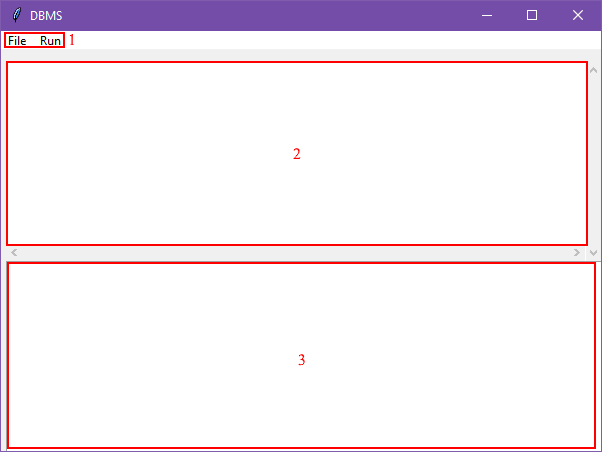
\includegraphics[width=1\linewidth]{images/interface}
	\caption{Макет рабочего окна программы}
	\label{fig:interface}
\end{figure}

Макет содержит следующие элементы:
\begin{enumerate}
	\item Главное меню
	
	Главное меню реализовано на основе виджета tk.Menu и состоит из двух основных разделов:
	\begin{itemize}
		\item File — содержит команды Save и Open для сохранения и загрузки базы данных из файла;
		\item Run — команда запуска обработки пользовательского ввода, выполняющей анализ текста, введённого в поле SQL-команды, и выполнение соответствующих операций.
	\end{itemize}
	Меню охватывает основные действия, необходимые для работы пользователя с базой данных, и остаётся доступным вне зависимости от текущего состояния приложения.
	
	\item Область отображения таблиц
	
	Эта часть интерфейса занимает верхнюю половину окна и реализована с помощью контейнера tk.Frame и виджета ttk.Treeview, предназначенного для отображения табличных структур в виде древовидной таблицы с колонками. Таблица автоматически подстраивается под содержимое и заполняет всё доступное пространство. Для удобства просмотра добавлены горизонтальная и вертикальная полосы прокрутки.
	
	При проведении операций над данными интерфейс обновляется динамически, подставляя актуальные данные в таблицу.
	
	\item Поле ввода команд
	
	В нижней части окна находится текстовое поле tk.Text, предназначенное для ввода пользователем команд на SQL-подобном языке. Это основная точка взаимодействия между пользователем и логическим ядром программы.
	
	По нажатию пункта Run введённая команда передаётся в модуль парсинга и обрабатывается соответствующим образом. Результат отображается либо в таблице, либо во всплывающем сообщении.
\end{enumerate}

Таким образом, интерфейс приложения предоставляет все необходимые средства для взаимодействия с табличными данными и служит оболочкой для логического ядра программы, выполняющего интерпретацию команд и управление данными.